\documentclass[conference]{IEEEtran}

\usepackage{cite}
\usepackage{amsmath,amssymb}
\usepackage{graphicx}
\usepackage{hyperref}
\usepackage{booktabs}
\usepackage{xcolor}

% Six-page condensation of paper.tex. Every reported number and every
% qualification is carried over; the prose is compressed and two figures
% carrying secondary results are dropped. See paper.tex for the full version.

\title{From Interpretable to Black-Box: Dynamic Model Identification
for Small USV Control Design}

\author{
  \IEEEauthorblockN{Brian S. Bingham and Carson Vogt}
  \IEEEauthorblockA{
    Department of Mechanical and Aerospace Engineering\\
    Naval Postgraduate School\\
    Monterey, CA, USA\\
    bbingham@nps.edu, crvogt@nps.edu
  }
}

\begin{document}
\maketitle

\begin{abstract}
Designing the low-level speed and heading loops of a small uncrewed surface vehicle (USV) requires a dynamic model, and it is rarely clear how much model the job needs. For vessels under seven meters with a single thruster and rudder, tow-tank testing is impractical and parameters must be identified from limited field trials. We treat sufficiency as a property of a stated design job, taking that job to be the proportional-integral plus feedforward stabilization loops of a production autopilot, and identify three model levels against that target: first-order linear SISO transfer functions, a nonlinear state-space form with quadratic drag, and a NARX multilayer perceptron. First-order models reach $R^2=0.93$ in surge and $R^2=0.83$ in yaw rate, enough to fix a PI+FF compensator. A margin-based test then reports where that model stops being good enough: a speed controller designed from it behaves as intended only between 0.35 and 1.28~m/s, since below that band the model error exceeds the stability margin and above it the loop stays stable but loses more than half its intended bandwidth. The NARX model reaches one-step $R^2=0.998$ in speed on a trial it never saw, yet falls to $-1.988$ under recursive simulation of that same trial, diverging in surge where both structured models stay bounded. One-step accuracy is a poor guide to simulation accuracy, and reporting it alone is not sufficient.
\end{abstract}

\begin{IEEEkeywords}
uncrewed surface vehicle, system identification, model spectrum, control-oriented modeling, robustness margin, underactuated vessels
\end{IEEEkeywords}

% ─────────────────────────────────────────────────────────────────────────────
\section{Introduction}
\label{sec:intro}

Small uncrewed surface vehicles, here vessels under seven meters driven by a single thruster and rudder, are increasingly deployed for survey, inspection and autonomy research. Every such mission rests on a working low-level controller: a speed loop on the throttle and a yaw-rate loop on the rudder, each holding a setpoint while a guidance layer above does the navigating. In production autopilots such as ArduPilot these are proportional-integral loops with an added feedforward term. Designing, simulating and tuning that pair of loops is the task this paper addresses, and the task against which every modeling decision below is judged.

The identification literature offers everything from two-parameter response models to maneuvering polynomials carrying dozens of hydrodynamic coefficients, but no guidance on which this job requires. Fixing the compensator structure makes the question answerable, because it turns concrete: does a change of model level move the gains, the achievable bandwidth or the tuning procedure of that loop? A model that alters none of the three is inert however much better it fits. Taking the most detailed model available is not a safe default either, since added terms degrade the conditioning of the fit~\cite{alexandersson2022system,suarez2026regularized} and each one needs excitation to identify, which converts fidelity directly into field trials on a platform where trials are the binding constraint. Sonnenburg and Woolsey~\cite{sonnenburg2013modeling} evaluate a cost function on held-out maneuvers, tabulate it per model and per regime, then select by judgment, discarding the best-scoring model because two extra parameters are not worth the slight edge. Their cost function scores the benefit of added parameters and no comparable metric exists for the cost, so the judgment has nothing to be replaced by. Skelton put the criterion in control terms in 1989, that model errors need not be small but only appropriate for the control design~\cite{skelton1989model}, and it has stood since without becoming computable.

Our scope is the single thruster plus rudder vessel with field-identified parameters. Underactuated rudder steering is the interesting case, because control authority is an explicit function of forward speed, so the steering and speed channels cannot be treated as independent design problems. We identify three model levels from common field data, compare them with cross-model diagnostics, and give a margin-based test reporting the speed range over which added fidelity stops changing the loop design. The deliverable is a procedure rather than a model: the diagnostics say which dynamics are present, and the margin test says which of them reach the compensator. Prior identification studies for this vehicle class compare candidate structures and then select one, after which the rest stop contributing; we keep the set. The models buy loop structure, verification in simulation, relative comparison of variants and a rehearsed tuning procedure. They do not buy gains that transfer without field tuning, and we say so plainly.

% ─────────────────────────────────────────────────────────────────────────────
\section{Closely Related Work}
\label{sec:related}

The minimal control-oriented description of a steered vessel is Nomoto's first-order steering model~\cite{nomoto1957steering}, still the standard starting point in the modern formulation~\cite{fossen2011handbook}, with the identification tradition founded by {\AA}str{\"o}m and K{\"a}llstr{\"o}m~\cite{astrom1976identification}. Physics-based maneuvering models such as Abkowitz's~\cite{abkowitz1964lectures} include coefficients with physical meaning but resist identification from field data: over the maneuvers a small vessel can realistically perform the regressors are nearly collinear, so many coefficient sets fit about equally well and none can be trusted on its own however well the model predicts as a whole~\cite{suarez2026regularized,alexandersson2022system,xu2025review}. For small craft the closest prior work is Sonnenburg and Woolsey~\cite{sonnenburg2013modeling,sonnenburg2010control}, with related efforts spanning autonomous surface craft and small workboats~\cite{eriksen2017modeling,muske2008identification,wirtensohn2013modelling,morel2025practical,sarda2016nmpc}.

Data-driven and grey-box marine models span recurrent architectures~\cite{woo2018dynamic}, physics-informed networks~\cite{xu2022pinn} and gradient-boosted ensembles~\cite{zhang2024gbm}, and our Level~3 follows the neural identification literature~\cite{narendra1990identification} and its delayed-input variants~\cite{lin1997delay}. The distinction relevant to control is between one-step prediction, which reads measured state history at every sample, and recursive simulation, which feeds predicted states back and is what a design loop requires. Reporting practice is uneven on this point, though Woo \emph{et al.}~\cite{woo2018dynamic} do validate through forward simulation. Three gaps follow: sufficiency is resolved by selecting one model rather than retaining the set, evaluation is inconsistent about the one-step versus recursive distinction, and the small rudder-steered vessel is underrepresented relative to differential-thrust research platforms.

% ─────────────────────────────────────────────────────────────────────────────
\section{Model Spectrum Methodology}
\label{sec:methodology}

Each level is judged by what it contributes to the PI-plus-feedforward loop of Sec.~\ref{sec:intro} rather than by goodness of fit: Level~1 settles the loop structure, Level~2 says where nonlinear feedforward is needed and Level~3 bounds what a black-box alternative would buy.

\emph{Level~1} treats surge and yaw as decoupled first-order channels, $G_v(s)=K_v/(\tau_v s+1)$ and $G_r(s)=K_r/(\tau_r s+1)$, mapping normalized throttle to speed and normalized rudder to yaw rate. Both are identified as discrete autoregressive models with exogenous input, ARX($n_a,n_b$) with $n_a=n_b=1$, so that $y(k)=a_1y(k-1)+b_1u(k-1)$, fitted by least squares on the 10~Hz record and converted to continuous time. $\tau$ is the open-loop pole the controller works against, so it sets the scale of closed-loop bandwidth worth asking for, and $K$ sets the loop gain. A PI structure follows, with internal model control tuning fixing its gains as $k_p=\tau/(K\lambda)$ and $k_i=1/(K\lambda)$ for a chosen closed-loop time constant $\lambda$.

\emph{Level~2} keeps the decoupled structure but replaces linear damping in surge with quadratic drag,
\begin{align}
\dot v &= k_T\,u - d_2\,v|v|, \label{eq:l2surge}\\
\dot r &= k_\delta\,\delta - d_r\,r. \label{eq:l2yaw}
\end{align}
Identification is two-phase. Fitting \eqref{eq:l2surge} jointly for $k_T$ and $d_2$ is poorly conditioned, because thrust and drag are large and nearly cancelling during steady runs, so the data constrains their difference far better than either term. Instead $d_2$ is estimated from coasting segments where $u=0$ and \eqref{eq:l2surge} reduces to $\dot v=-d_2v|v|$, then $k_T$ follows from the powered segments. The yaw channel keeps a constant $k_\delta$, which is a local approximation rather than a physical claim: rudder force grows with the square of flow speed, so $k_\delta$ must vary with forward speed, and the value identified here holds near the speed at which the rudder steps were flown.

\emph{Level~3} is a fixed-tap residual NARX multilayer perceptron with 19 lagged inputs, one hidden layer of 64 tanh units and two outputs which are state increments rather than absolute states. State history extends 0.5~s into the past, throttle history 2~s and rudder history 1~s. The lag structure is a project-specific choice consistent with delayed-input NARX models~\cite{lin1997delay}. Being multi-input multi-output, it is free to discover the surge-yaw coupling absent in Levels~1 and~2. It is a compact black-box reference point and no claim is made that this architecture is optimal.

\subsection{Evaluation Protocol}

Two scores are reported and they are not interchangeable. One-step prediction advances the model a single sample from measured state history, so every prediction begins from the truth. Recursive simulation initializes once from measured history, then feeds the model's own output back as its state while replaying the throttle and rudder actually recorded, and runs to the end of the segment without further correction. Level~3 initializes from 2~s of measured history, the span of its longest input tap; the structured levels need one sample. No controller is present in either case: the commands are those the operator or autopilot issued during the trial, replayed open loop, so recursive simulation asks whether the model can stand in for the vehicle, not how a control loop behaves. Fit is reported per channel as $R^2 = 1-\sum_k(y_k-\hat y_k)^2/\sum_k(y_k-\bar y)^2$, so zero is the score of predicting the channel mean and negative values are worse than that.

\subsection{Cross-Model Diagnostics}

The value of the spectrum is the comparison across levels rather than the three fits individually. Scoring one structure on held-out data is a weaker check here, because a maneuvering model can pass a prediction test while its coefficients remain physically meaningless~\cite{alexandersson2022system}, and a coefficient that cannot be interpreted cannot inform a control gain. The four diagnostics are not an arbitrary list: Levels~1 and~2 differ in exactly one term, the form of the surge damping, and share exactly two simplifying assumptions, that the channels are decoupled and that rudder authority does not vary with speed. One diagnostic tests the term that separates the levels, two test the shared assumptions, and the fourth asks whether any of it reaches the compensator.

\emph{Diagnostic 1, speed-dependent rudder gain.} Replace the constant $k_\delta$ in \eqref{eq:l2yaw} with a speed-scaled $k_\delta v$ and test whether the yaw-rate fit improves. Gain scheduling is well within a production autopilot's capability, so the question is not whether the controller can accommodate the effect but whether the model can say what schedule to use; a constant $k_\delta$ cannot. The alternative tested is partial, since Nomoto scaling gives $k_\delta\propto v^2$ with $d_r\propto v$~\cite{fossen2011handbook} while the regression scales only the input gain and only linearly.

\emph{Diagnostic 2, drag nonlinearity.} The form of the surge damping is the only structural difference between Levels~1 and~2, so this is the warrant for Level~2 existing at all. Fit linear and quadratic damping to the coasting deceleration and compare. A dominant quadratic term calls for nonlinear feedforward on the speed loop.

\emph{Diagnostic 3, rudder-induced surge drag.} The reverse coupling to Diagnostic~1; together they test decoupling in both directions. Correlate $\delta^2$ against the surge residual of the Level-2 fit. A correlation would make every rudder command a disturbance to the speed loop.

\emph{Diagnostic 4, is the added fidelity inside the robustness margin?} The first three ask whether a term is real; this asks whether a real term changes the design. The robustness margin of a compensator is a budget for model error, so the test is whether the Level-1 to Level-2 discrepancy fits inside the margin of a controller designed from Level~1 alone. Design a nominal internal model control PI from Level~1 only, $C(s)=(\tau_v s+1)/(K_v\lambda s)$, giving a nominal loop $L=1/(\lambda s)$ and complementary sensitivity $T(s)=1/(\lambda s+1)$. Linearizing Level~2 about $v_0>0$, where $\partial(v|v|)/\partial v=2v_0$, gives a speed-scheduled first-order plant
\begin{equation}
G_2(s,v_0)=\frac{K_2(v_0)}{\tau_2(v_0)s+1},\quad
\tau_2=\frac{1}{2d_2v_0},\quad K_2=\frac{k_T}{2d_2v_0},
\label{eq:lin}
\end{equation}
in which gain and time constant both fall as $1/v_0$. Form the multiplicative error $\ell(\omega,v_0)=|G_2(j\omega,v_0)/G_1(j\omega)-1|$ and test robust stability, $\|\ell T\|_\infty<1$. That test alone proves insufficient: quadratic drag is stabilizing, so at high speed the Level-1 design becomes sluggish rather than unstable and the stability test keeps passing. We therefore add a performance criterion, comparing the achieved closed-loop bandwidth of the Level-1 compensator on $G_2(s,v_0)$ against the design intent $1/\lambda$. The pair bounds sufficiency from both sides.

% ─────────────────────────────────────────────────────────────────────────────
\section{Experimental Platform and Data}
\label{sec:experiment}

\begin{figure}[t]
  \centering
  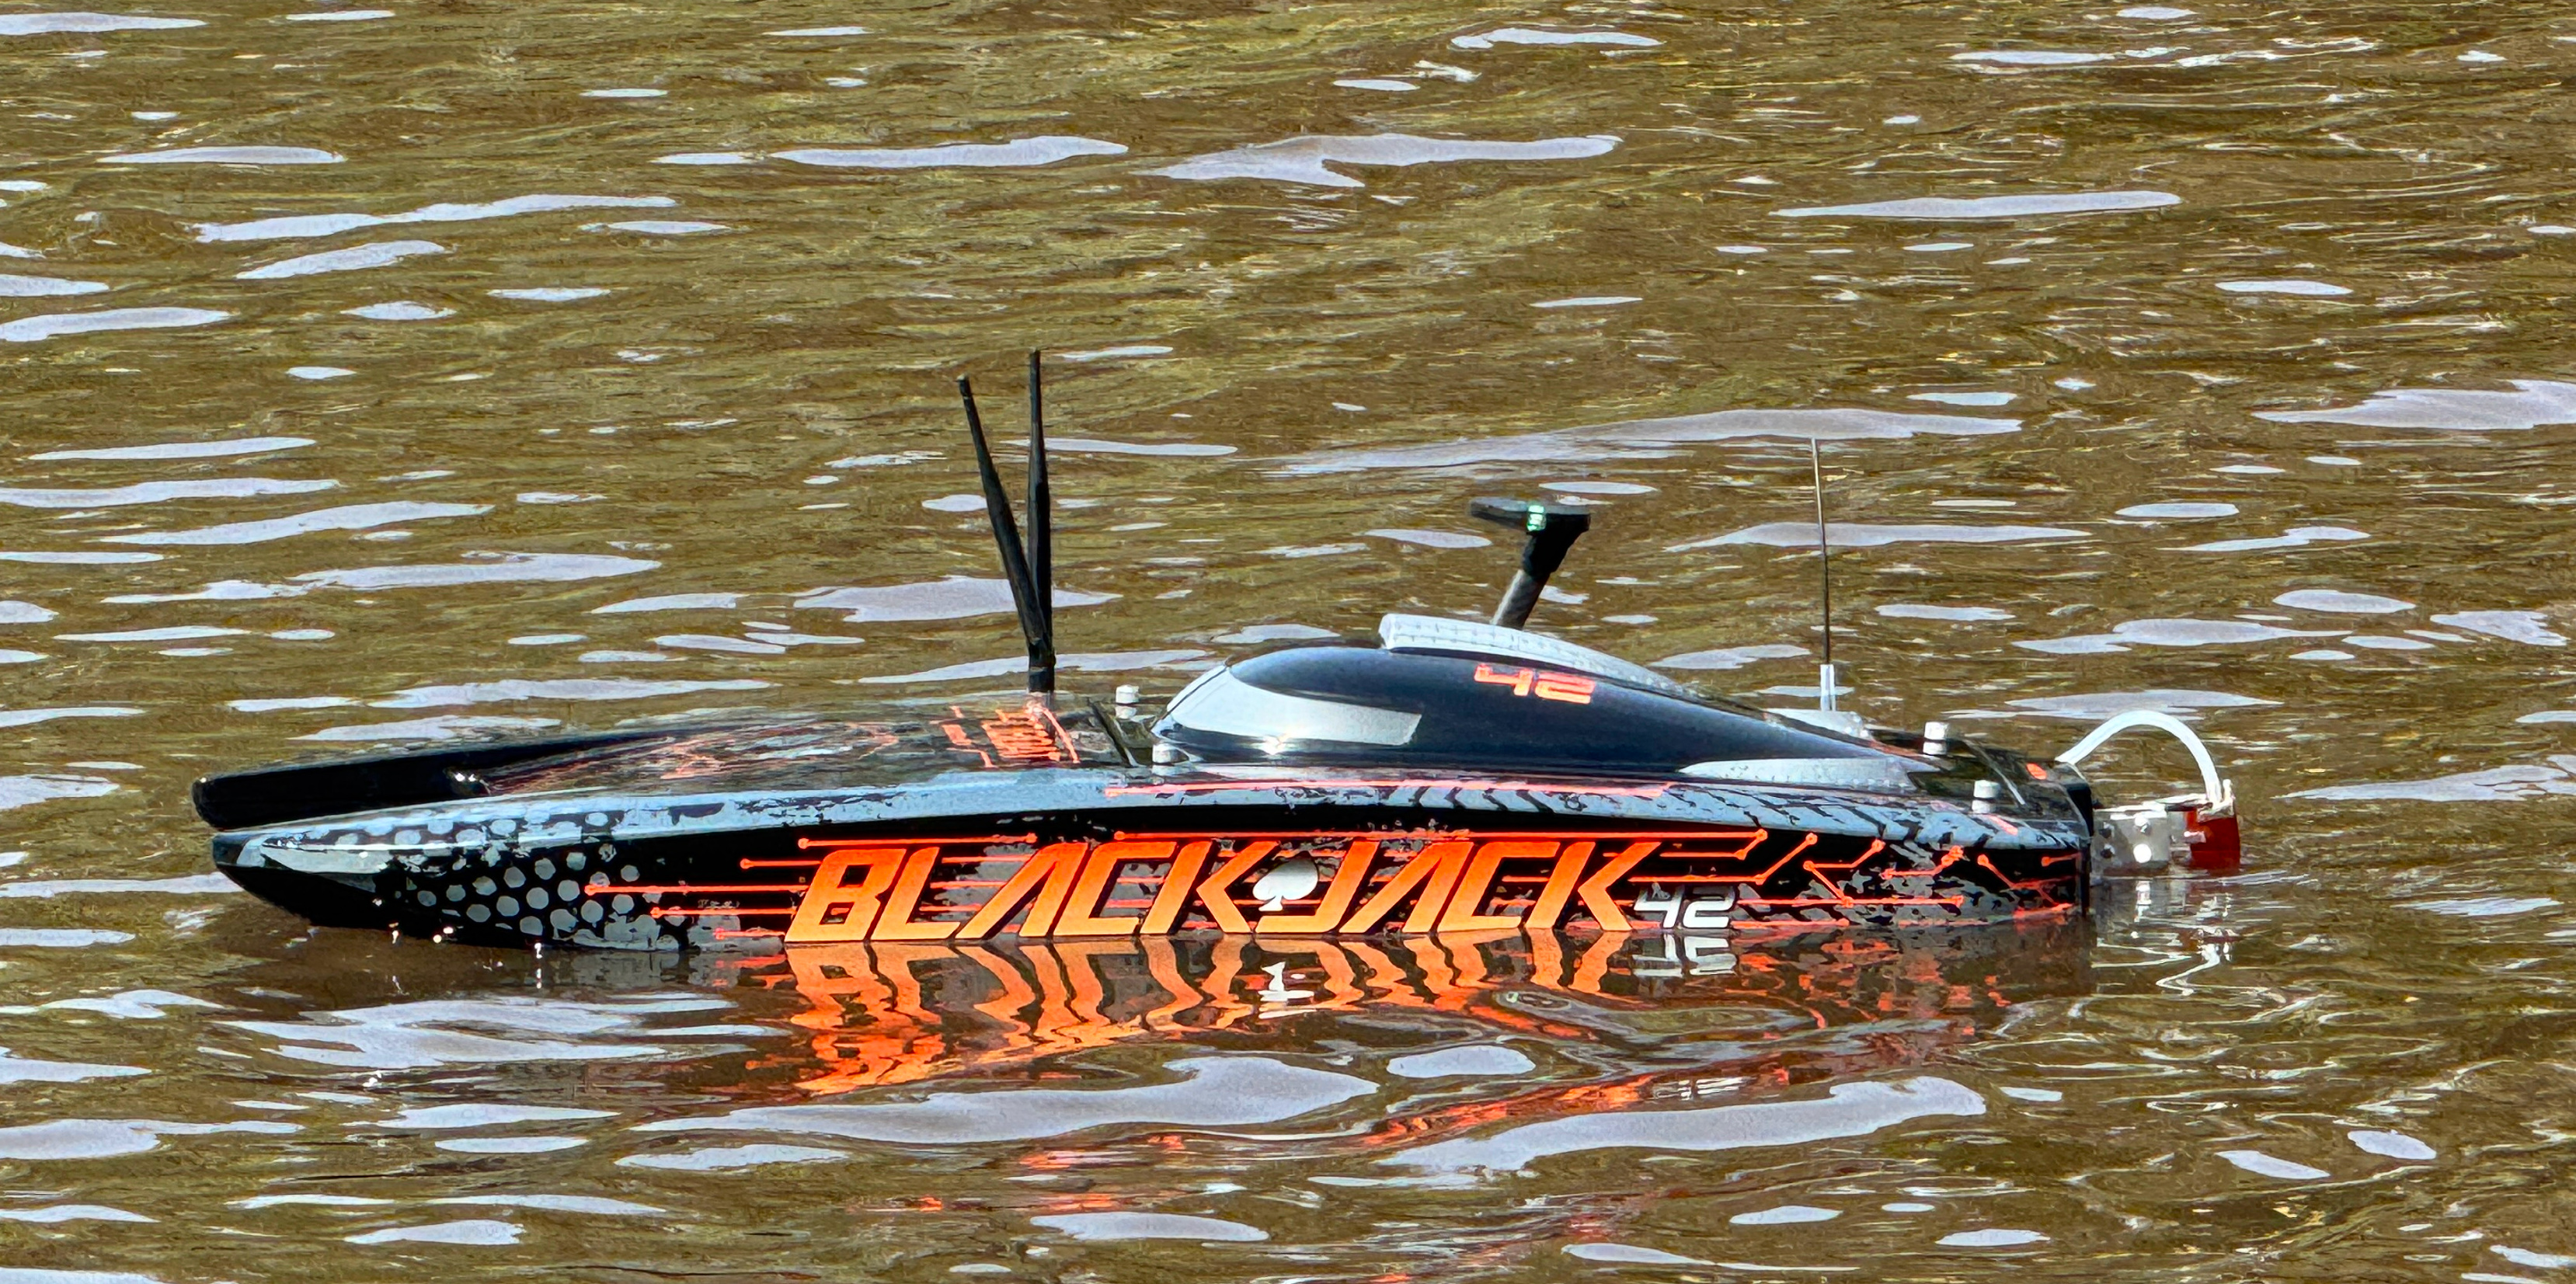
\includegraphics[width=\columnwidth]{images/blackjack42_usv.JPG}
  \caption{The experimental platform, a Pro Boat Blackjack 42 monohull of 1.07~m length. Thrust comes from a single propeller and steering from a single rudder, both at the stern.}
  \label{fig:platform}
\end{figure}

The platform (Fig.~\ref{fig:platform}) is a Pro Boat Blackjack 42, a production radio-controlled monohull of 1.07~m length instrumented to approximately 5~kg. Propulsion is single-screw: one water-cooled brushless motor turning a single propeller, with a single rudder on one digital servo. Guidance, control and logging run on a Cube Orange executing ArduRover 4.6.3, with position and ground speed from a HERE3 GNSS receiver. The parameter set confirms the actuation: \texttt{SERVO1} is assigned to ground steering and \texttt{SERVO3} to throttle, every other output disabled, so there is no differential-thrust path. Commands are logged as \texttt{RCOU\_C3} and \texttt{RCOU\_C1} at 1100--1900~$\mu$s PWM and normalized to $[-1,1]$ about the 1500~$\mu$s neutral point; outputs are \texttt{GPS\_Spd} at 5~Hz and \texttt{IMU\_GyrZ} at 137~Hz. Trials are flown in manual mode, so logged commands are open-loop operator inputs. The autopilot's stabilization layer is the design target: two loops, \texttt{ATC\_SPEED\_*} and \texttt{ATC\_STR\_RAT\_*}, each nominally a PID with feedforward, with derivative gain set to zero on this vehicle so the deployed compensator is PI plus feedforward. The configured cruise speed is 5~m/s, so the identification trial below covers roughly the lower half of the intended speed range.

Multi-rate streams are aligned to a common 10~Hz grid by linear interpolation, and records segmented at mode changes and quality discontinuities. Levels~1 and~2 are identified from a single step-response trial: a 130~s window from a 341~s recording, throttle 0--39\%, speed 0--2.9~m/s, 1{,}300 samples, with one 29.3~s repositioning gap handled by segmentation. Level~3 draws on a larger corpus of 44{,}133 samples in 70 slow-region segments from 65 source logs, where the slow-region rule excludes a segment once speed stays above 3.4028~m/s for at least 1~s. Allocation is grouped by source log. Training uses 37 logs, 40 segments and 28{,}023 rows. The remaining 28 logs, 30 segments and 16{,}110 rows are pooled for evaluation, and that pool needs describing accurately rather than as a held-out set: it combines 8 logs used for early stopping and hyperparameter selection, 9 used to choose among model families, and 11 nominally reserved as a closed test set that was opened before the checkpoint was fixed. The checkpoint was selected manually after that evaluation rather than by the pre-declared rule, so metrics on this pool are optimistic and we treat them as descriptive. The frozen Level~3 model is additionally evaluated on the same 130~s trial used for Levels~1 and~2. That trial is not part of the Level-3 corpus, confirmed by cross-correlating it against every corpus segment, so it is unseen by Level~3 while Levels~1 and~2 are identified from it. Its 20-sample lag history leaves 1{,}279 scored rows against 1{,}300.

% ─────────────────────────────────────────────────────────────────────────────
\section{Results}
\label{sec:results}

Least squares on the step-response trial gives $G_v(s)=6.42/(1.95s+1)$ and $G_r(s)=0.771/(0.471s+1)$, with simulation $R^2=0.930$ in surge and $0.826$ in yaw rate. These are in-sample figures: the trial is short enough that withholding part of it would leave too little excitation to identify against, so fit and score both use all 1{,}300 samples, and the same holds for Level~2. The surge and yaw time constants differ by a factor of four, which alone settles the loop structure.

Two-phase identification gives $\dot v = 3.963\,u - 0.438\,v|v|$ and $\dot r = 1.474\,\delta - 1.912\,r$, with $R^2=0.909$ in surge and $0.820$ in yaw rate. Both sit marginally below Level~1 on this trial, which is expected, since Level~1 minimizes exactly this error on exactly this data while Level~2 takes its drag coefficient from coasting alone. The useful comparison is what the structure exposes.

\subsection{Level 3}
\label{sec:l3-results}

On the 30-segment evaluation pool the one-step macro-NRMSE is 0.084 and the recursive macro-NRMSE is 0.425; speed $R^2$ falls from 0.998 one-step to 0.836 recursive, and yaw-rate $R^2$ from 0.991 to 0.768. On the common trial Level~3 reaches one-step $R^2$ of 0.998 in speed and 0.989 in yaw rate, and under recursive simulation falls to $-1.988$ and $0.259$. Fig.~\ref{fig:combined} shows the surge trajectory drifting below zero and staying there for tens of seconds.

The result we claim is the gap between one-step and recursive prediction, not the ranking of the three levels. That gap is measured within a single model on identical data, so it is unaffected by how the models were fitted. One-step prediction reads the measured state at every sample, so a model can score 0.998 while having learned little more than that the state changes slowly; recursive simulation removes that support and the per-step increment errors accumulate. The same gap appears on the evaluation pool, so it is a property of the model rather than of one trial.

The apparent ranking in Fig.~\ref{fig:combined} will not carry that weight. Levels~1 and~2 are scored on the trial they were identified from while Level~3 is scored on a trial it never saw, so part of the separation is the ordinary in-sample advantage rather than an effect of model structure. We make no quantitative claim that structure outperforms the black box. What the figure establishes is that the structured models stay bounded while the black box does not, which follows from the drag term rather than from the fit.

\begin{figure}[t]
  \centering
  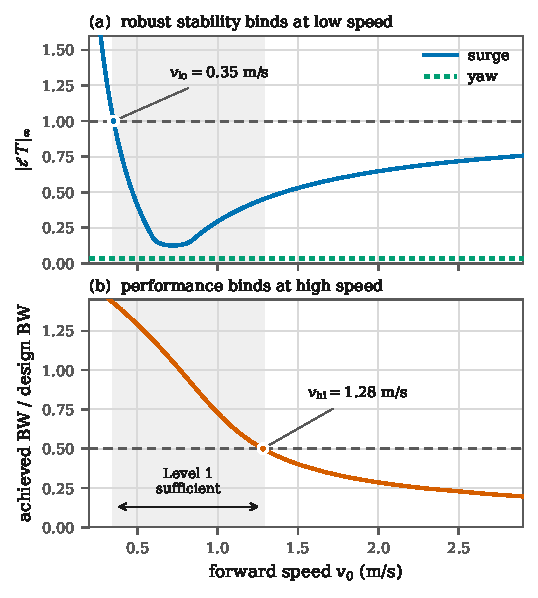
\includegraphics[width=\columnwidth]{figures/diagnostic4_margin.pdf}
  \caption{Diagnostic~4. (a) Robust stability of the Level-1 compensator against the Level-2 linearization binds at low speed, where the quadratic-drag linearization is singular. (b) Achieved closed-loop bandwidth binds at high speed. The shaded band is the interval over which the Level-1 model supports the design. The yaw channel (a, dotted) never approaches the limit.}
  \label{fig:diagnostic4}
\end{figure}

\subsection{Cross-Model Diagnostic Summary}
\label{sec:diag-results}

\emph{Diagnostic 1} finds no improvement from a speed-dependent rudder gain ($\Delta R^2=-0.03$). The trial holds forward speed nearly constant during the rudder steps, so $\delta v$ and $\delta$ are very nearly the same regressor, with a correlation of 0.99, and no fit can separate them; the partial scaling noted above is a second candidate explanation. Repeating the diagnostic across a supplementary set of manual-mode records confirms the attribution: the improvement from the speed-scaled gain tracks how far speed varies while the rudder is deflected, and the clearest record, holding rudder from 0.46 to 4.48~m/s, returns $\Delta R^2=+0.13$. Averaged over those records the improvement is only $+0.02$ and the fits are in-sample, so the effect is not thereby established. What is established is what the rudder sweeps must achieve: not more data, but rudder applied across separated speeds.

\emph{Diagnostic 2} finds quadratic damping dominant, with $\Delta R^2=+0.20$ over the linear fit, $d_1=-0.015$ and $d_2=0.448$~m$^{-1}$ on the coasting segments. The two-phase identification returns $d_2=0.438$~m$^{-1}$ from the same segments under the Level-2 parameterization, a weak consistency check rather than an independent one.

\emph{Diagnostic 3} finds rudder-induced surge drag negligible, with a correlation of $r=-0.08$ between $\delta^2$ and the surge residual. The coupling term is not warranted.

\emph{Diagnostic 4} is reported in Fig.~\ref{fig:diagnostic4}, computed with $\lambda=1.0$~s, and returns an interval rather than a threshold. Robust stability fails below $v_0=0.35$~m/s, a bound with the closed form $v_{\text{lo}}=k_T/(4d_2K_v)$, independent of $\lambda$ because $|T|\leq1$ places the supremum of $\ell|T|$ at DC. The mechanism is the $1/v_0$ singularity in \eqref{eq:lin}: quadratic drag provides no linear damping at zero speed. At the upper end the stability test never fails, and at 2.9~m/s the model error is still within budget at $\|\ell T\|_\infty=0.76$. What fails is performance: the Level-1 compensator on the Level-2 plant retains only 20\% of its intended bandwidth at 2.9~m/s, crossing 50\% at $v_{\text{hi}}=1.28$~m/s. The two bounds are not equally firm. The lower follows from $\|\ell T\|_\infty=1$; the upper depends on choosing 50\% of design bandwidth as the point where degradation becomes unacceptable, which is a convention rather than a result, since a 70\% criterion moves it to 1.03~m/s and a 30\% criterion to 1.91~m/s. Both are insensitive to $\lambda$: sweeping it from 0.5 to 3~s moves $v_{\text{hi}}$ only between 1.23 and 1.61~m/s. For yaw, Level~2 linearizes to $0.771/(0.523s+1)$ against Level~1's $0.771/(0.471s+1)$, identical DC gain and an 11\% difference in time constant, giving $\|\ell T\|_\infty=0.034$. Level~2 buys nothing for yaw control across the whole envelope.

\begin{figure*}[t]
  \centering
  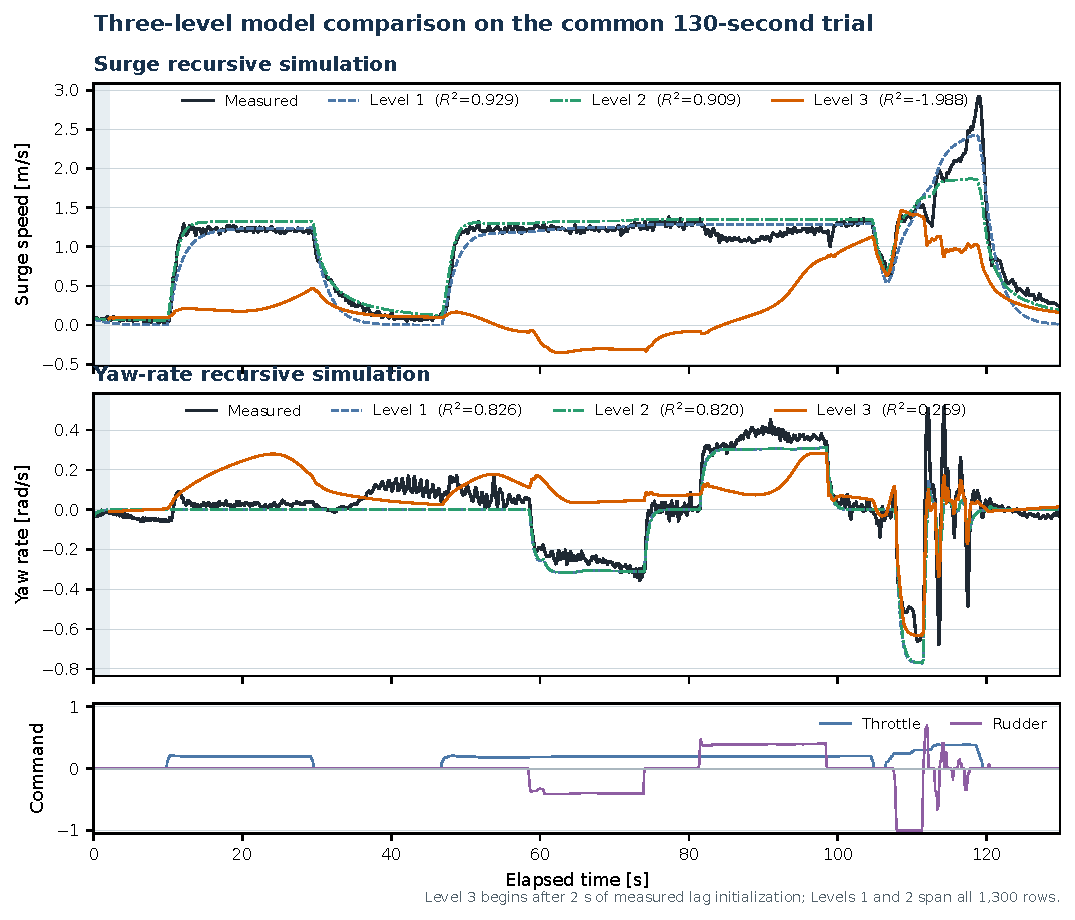
\includegraphics[width=\textwidth]{figures/preview/combined_three_level_preview.pdf}
  \caption{All three levels under recursive simulation on the common 130~s trial. Levels~1 and~2 track the measured response; Level~3 diverges in surge, driving predicted speed below zero for tens of seconds despite the highest one-step accuracy of the three. Level~3 begins after 2~s of measured lag initialization, so it scores 1{,}279 rows against 1{,}300 for Levels~1 and~2.}
  \label{fig:combined}
\end{figure*}

% ─────────────────────────────────────────────────────────────────────────────
\section{Discussion}
\label{sec:discussion}

For this vehicle at the speeds tested, surge and yaw are weakly coupled, so decoupled SISO controllers are a defensible starting point. Quadratic drag is significant, so a speed-hold controller needs nonlinear feedforward and a purely linear one will show speed-dependent steady-state error. Whether the rudder gain scales with speed can be neither confirmed nor denied from the identification trial. No single model exposes all of this: Level~1 gives no reason to suspect the drag is quadratic, Level~2 does not reveal that its extra structure is inert for yaw, and Level~3 alone would report an excellent one-step score and mislead anyone who took it to simulation.

Level~1 supports a baseline PI with directly identified gains, valid over the interval Diagnostic~4 returns. Level~2 justifies nonlinear feedforward on the surge channel and says at what speed it becomes necessary; on yaw it changes nothing, so the added structure should not be carried into the design. Level~3 bounds what lies beyond the fixed architecture: a black-box model free to discover the coupling the structured levels assume away is the natural precursor to model-predictive or learning-based control, and its recursive failure says the data does not yet support moving past PI plus feedforward. None of the three delivers gains that work on the water without adjustment. What the spectrum buys is the loop structure, a simulation to verify it in, a basis for comparing variants and a tuning session that can be planned rather than improvised.

It is tempting to read the Level-3 result as showing that physical structure beats data volume, since Level~3 saw 28{,}023 training samples against the 1{,}300 used for Levels~1 and~2 and still simulated worst. We do not make that claim: the levels were fitted and scored under different protocols, so the comparison cannot separate the contribution of structure from that of sampling, and the sensitivity of each level to training-set size is unmeasured here.

\emph{Limitations.} Levels~1 and~2 rest on a single trial covering 0--2.9~m/s and throttle to 39\%, so the identified parameters are not a characterization across the envelope, and Diagnostic~4 inherits that limitation. The common-trial comparison rests on one 130~s record, enough to demonstrate the divergence but not to quantify how often it occurs. Level~3's corpus is restricted to the slow region by construction, so nothing here speaks to behavior near the planing transition, and with a configured cruise speed of 5~m/s no level is characterized over the upper half of the intended range. All results come from a single vehicle.

% ─────────────────────────────────────────────────────────────────────────────
\section{Conclusion}
\label{sec:conclusion}

We have presented a three-level model spectrum for small underactuated USVs, identified from field trials and posed throughout against one concrete question: what does a practitioner need in order to design, simulate and tune the speed and yaw-rate loops of a production autopilot? The spectrum collectively answers that question better than any single model does, and simple models are a persistent tool for this work rather than a stepping stone. The margin-based test converts Skelton's qualitative criterion into a computed interval, returning $[0.35, 1.28]$~m/s for the surge channel and reporting that the same test is satisfied everywhere on the yaw channel, where the added Level-2 structure is inert.

Future work runs in three directions. The first is data: dedicated rudder sweeps at separated fixed speeds, which is what breaks the collinearity Diagnostic~1 could not overcome. The second is a stronger basis for cross-level comparison, since the present common trial is a single record and a multi-trial evaluation set would let the Level-3 divergence be quantified rather than demonstrated; the sensitivity of each level to training-set size belongs here too. The third is to treat the robustness margin as a formal sufficiency criterion across the spectrum, computing for each design decision the level at which further fidelity is provably inert, replacing expert judgment with a computable bound on how much model a given autopilot loop requires.

\bibliographystyle{IEEEtran}
\bibliography{references}

\end{document}
